\scanpage{2}
\figure{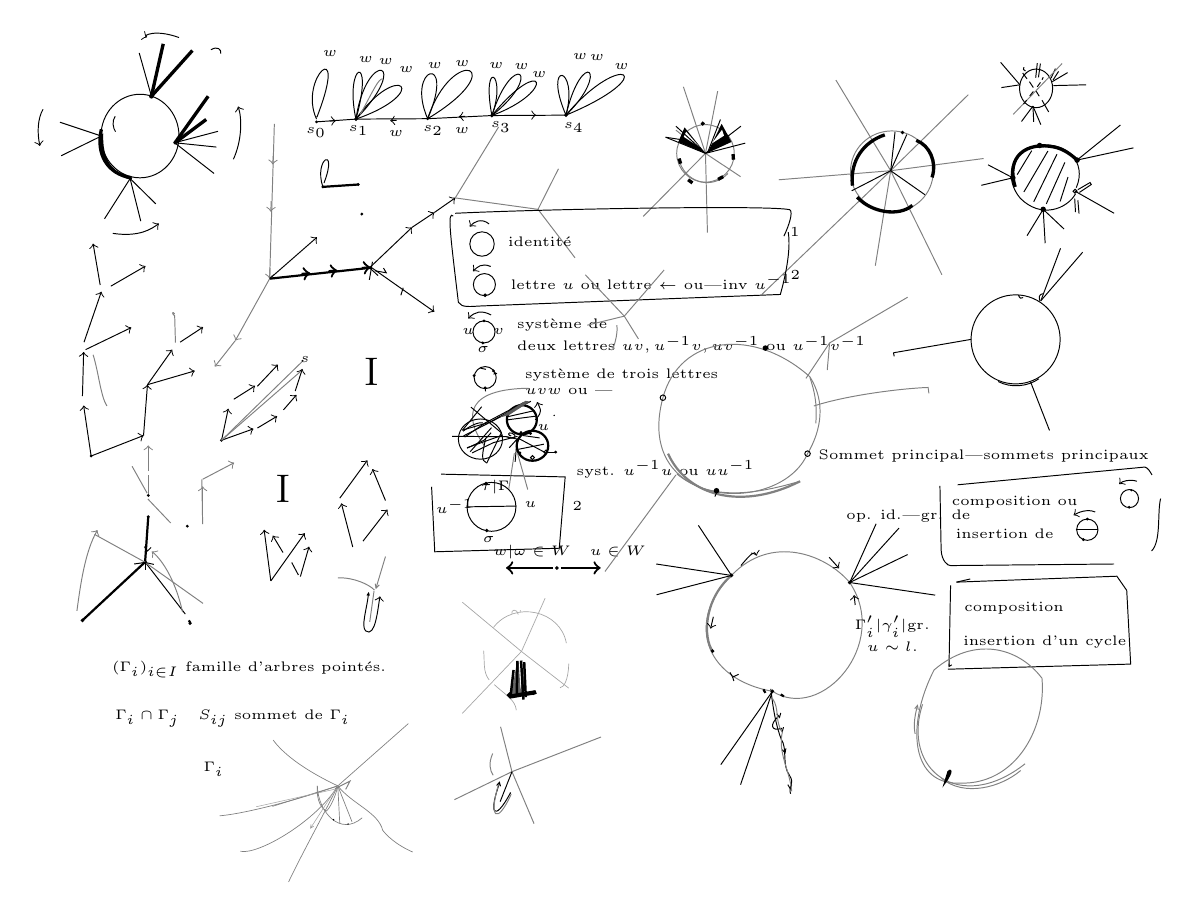
\begin{tikzpicture}[x=.005cm,y=-.005cm,line width=.35pt,every node/.style={font=\tiny,inner sep=1pt}]
\path[use as bounding box] (105,20) rectangle (2990,2218);
% G01: upper-left wheel
\draw (390,295) ellipse (99 and 106); % G01.circ
\draw[very thick] (292,278) .. controls (278,340) and (306,391) .. (368,401); % G01.over1
\draw[thick] (294,289) .. controls (291,353) and (316,392) .. (369,403); % G01.over2
\draw (327,245) .. controls (318,257) and (322,276) .. (328,284); % G01.inner
\draw[very thick] (419,194)--(449,61); % G01.top1
\draw[very thick] (419,194)--(523,78); % G01.top2
\draw (419,194)--(388,84); % G01.top3
\draw (292,295)--(187,260); % G01.left1
\draw (292,295)--(190,345); % G01.left2
\draw[very thick] (479,312)--(563,194); % G01.right1
\draw[very thick] (479,312)--(558,253); % G01.right2
\draw (478,312)--(588,283); % G01.right3
\draw (478,312)--(584,323); % G01.right4
\draw (478,312)--(578,390); % G01.right5
\draw (365,403)--(300,505); % G01.bottom1
\draw (365,403)--(392,511); % G01.bottom2
\draw (365,403)--(430,467); % G01.bottom3
\fill (419,194) circle(6); % G01.pttop
\fill (479,312) circle(5); % G01.ptright
\fill (292,295) circle(4); % G01.ptleft
\fill (365,403) circle(5); % G01.ptbottom
\draw[->] (489,45) .. controls (428,23) and (398,40) .. (408,44); % G01.rot_top
\draw[->] (144,227) .. controls (130,251) and (129,287) .. (136,320); % G01.rot_left
\draw[->] (321,542) .. controls (390,552) and (420,530) .. (438,517); % G01.rot_bottom
\draw[->] (627,354) .. controls (649,306) and (649,250) .. (639,220); % G01.rot_right
\draw (570,76) .. controls (587,66) and (597,75) .. (595,86); % G01.isolated
% G02: five-vertex loop chain
\fill (838,259) circle(4); % G02.s0_point
\fill (938,252) circle(5); % G02.s1_point
\fill (1120,251) circle(4); % G02.s2_point
\fill (1283,243) circle(5); % G02.s3_point
\fill (1471,242) circle(5); % G02.s4_point
\draw (838,259)--(938,252); % G02.edge1
\draw (1120,251)--(938,252); % G02.edge2
\draw (1283,243)--(1120,251); % G02.edge3
\draw (1283,243)--(1471,242); % G02.edge4
\draw[->] (871,257)--(887,256); % G02.head1
\draw[->] (1041,255)--(1025,256); % G02.head2
\draw[->] (1215,245)--(1199,246); % G02.head3
\draw[->] (1379,242)--(1395,242); % G02.head4
\draw (838,252) .. controls (790,147) and (923,31) .. (839,247); % G02.s0a
\draw (938,252) .. controls (907,109) and (987,78) .. (938,252); % G02.s1a
\draw (938,252) .. controls (965,71) and (1083,103) .. (938,252); % G02.s1b
\draw (938,252) .. controls (1048,99) and (1133,184) .. (938,252); % G02.s1c
\draw (1120,251) .. controls (1062,118) and (1194,80) .. (1120,251); % G02.s2a
\draw (1120,251) .. controls (1184,58) and (1339,119) .. (1120,251); % G02.s2b
\draw (1283,243) .. controls (1255,94) and (1323,134) .. (1283,243); % G02.s3a
\draw (1283,243) .. controls (1336,74) and (1419,135) .. (1283,243); % G02.s3b
\draw (1283,243) .. controls (1416,81) and (1451,181) .. (1283,243); % G02.s3c
\draw (1471,242) .. controls (1410,100) and (1505,115) .. (1471,242); % G02.s4a
\draw (1471,242) .. controls (1512,68) and (1587,128) .. (1471,242); % G02.s4b
\draw (1471,242) .. controls (1613,73) and (1718,139) .. (1471,242); % G02.s4c
\node at (872,85) {$w$}; % G02.w01
\node at (963,102) {$w$}; % G02.w02
\node at (1014,107) {$w$}; % G02.w03
\node at (1066,125) {$w$}; % G02.w04
\node at (1138,115) {$w$}; % G02.w05
\node at (1208,111) {$w$}; % G02.w06
\node at (1294,116) {$w$}; % G02.w07
\node at (1358,118) {$w$}; % G02.w08
\node at (1403,140) {$w$}; % G02.w09
\node at (1507,92) {$w$}; % G02.w10
\node at (1550,95) {$w$}; % G02.w11
\node at (1612,118) {$w$}; % G02.w12
\node at (1040,289) {$w$}; % G02.w13
\node at (1207,282) {$w$}; % G02.w14
\node at (837,286) {$s_{0}$}; % G02.s0_label
\node at (945,282) {$s_{1}$}; % G02.s1_label
\node at (1134,281) {$s_{2}$}; % G02.s2_label
\node at (1306,272) {$s_{3}$}; % G02.s3_label
\node at (1491,273) {$s_{4}$}; % G02.s4_label
\draw[gray] (949,240) .. controls (980,184) and (995,148) .. (1006,150); % G02.faint_return01
% G03: small loop and edge with isolated point
\draw (854,424) .. controls (830,351) and (894,318) .. (857,414); % G03.loop
\draw[thick] (854,424)--(944,418); % G03.edge
\fill (854,424) circle(4); % G03.junction
\fill (944,418) circle(4); % G03.right
\fill (953,493) circle(4); % G03.isolated
% G04: pale wheel with dark sectors
\draw[gray] (1769,170)--(1825,339); % G04.pencil1
\draw[gray] (1825,339)--(1830,540); % G04.pencil2
\draw[gray] (1856,181)--(1825,339); % G04.pencil3
\draw[gray] (1825,339)--(1667,499); % G04.pencil4
\draw[gray] (1825,339)--(1750,280); % G04.pencil5
\draw[gray] (1825,339)--(1914,398); % G04.pencil6
\draw[gray] (1825,339) ellipse (73 and 73); % G04.circ
\draw[gray] (1760,363) .. controls (1781,418) and (1845,429) .. (1882,390); % G04.over
\draw[very thick] (1815,261)--(1821,266); % G04.tick1
\draw[very thick] (1758,352)--(1762,365); % G04.tick2
\draw[very thick] (1781,406)--(1792,414); % G04.tick3
\draw[very thick] (1857,405)--(1870,398); % G04.tick4
\draw[very thick] (1895,341)--(1896,355); % G04.tick5
\fill (1825,339)--(1772,273)--(1756,310)--cycle; % G04.sectorL
\fill[white] (1810,323)--(1776,284)--(1770,297)--cycle; % G04.gapL
\fill (1830,338)--(1866,264)--(1891,310)--cycle; % G04.sectorR
\fill[white] (1841,314)--(1867,279)--(1872,294)--cycle; % G04.gapR
\draw (1825,339)--(1724,298); % G04.ink1
\draw (1724,298)--(1775,306); % G04.ink2
\draw (1825,339)--(1750,270); % G04.ink3
\draw (1830,338)--(1863,253); % G04.ink4
\draw (1825,339)--(1915,270); % G04.ink5
\draw (1825,339)--(1926,313); % G04.ink6
% G05: three-arc wheel
\draw[gray] (2295,383)--(2156,153); % G05.pencil1
\draw[gray] (2295,383)--(2492,190); % G05.pencil2
\draw[gray] (2295,383)--(2531,352); % G05.pencil3
\draw[gray] (2295,383)--(2425,647); % G05.pencil4
\draw[gray] (2295,383)--(2256,624); % G05.pencil5
\draw[gray] (2295,383)--(1968,697); % G05.pencil6
\draw[gray] (2295,383)--(2011,406); % G05.pencil7
\draw[gray] (2298,385) ellipse (105 and 103); % G05.pale_circ
\draw[very thick] (2198,421) .. controls (2191,356) and (2228,309) .. (2280,292); % G05.arc1
\draw[very thick] (2360,306) .. controls (2394,319) and (2413,360) .. (2400,400); % G05.arc2
\draw[very thick] (2210,450) .. controls (2247,490) and (2316,500) .. (2350,471); % G05.arc3
\fill (2396,340) circle(3); % G05.arc_return
\draw (2295,383)--(2196,434); % G05.ink1
\draw (2295,383)--(2382,444); % G05.ink2
\draw (2295,383)--(2306,285); % G05.ink3
\draw (2295,383)--(2336,291); % G05.ink4
\fill (2325,286) circle(5); % G05.topdot
% G06: small ray circle at top right
\draw (2664,174) ellipse (42 and 49); % G06.circ
\draw (2623,165)--(2574,108); % G06.ray1
\draw (2623,165)--(2576,172); % G06.ray2
\draw (2705,157)--(2744,134); % G06.ray3
\draw (2708,167)--(2791,165); % G06.ray4
\draw (2656,219)--(2627,258); % G06.ray5
\draw (2656,219)--(2676,266); % G06.ray6
\draw (2656,219)--(2658,259); % G06.ray7
\draw (2663,147)--(2667,110); % G06.tick1
\draw (2670,146)--(2675,111); % G06.tick2
\draw (2702,148)--(2713,124); % G06.tick3
\draw (2707,153)--(2721,131); % G06.tick4
\draw[gray] (2606,240)--(2730,111); % G06.faint_diag
\draw (2630,135)--(2641,150); % G06.fragment1
\draw (2647,157)--(2657,172); % G06.fragment2
\draw (2664,181)--(2672,194); % G06.fragment3
\draw (2679,204)--(2696,234); % G06.fragment4
\draw (2632,214)--(2640,204); % G06.fragment5
\draw (2648,193)--(2657,182); % G06.fragment6
\draw (2667,170)--(2675,159); % G06.fragment7
\draw (2679,152)--(2682,146); % G06.fragment8
\draw (2633,120) .. controls (2630,125) and (2632,128) .. (2637,130); % G06.tiny_curl
% G07: hatched five-mark disc
\draw (2766,426) .. controls (2794,361) and (2741,309) .. (2673,319) .. controls (2593,330) and (2584,407) .. (2624,453) .. controls (2677,506) and (2742,480) .. (2764,442); % G07.circ
\draw[very thick] (2611,424) .. controls (2586,346) and (2640,308) .. (2711,323) .. controls (2734,328) and (2753,342) .. (2768,356); % G07.over
\fill (2605,401) circle(7); % G07.pt_left
\fill (2673,319) circle(7); % G07.pt_top
\fill (2768,356) circle(7); % G07.pt_upperright
\fill (2682,481) circle(7); % G07.pt_bottom
\draw (2763,435) circle(5); % G07.ring
\draw (2605,401)--(2542,368); % G07.left1
\draw (2605,401)--(2525,420); % G07.left2
\draw (2768,356)--(2878,267); % G07.rightup1
\draw (2768,356)--(2911,325); % G07.rightup2
\draw (2770,431)--(2801,413)--(2804,418)--(2774,438); % G07.short1
\draw (2763,435)--(2862,491); % G07.longright
\draw (2682,481)--(2641,548); % G07.bottom1
\draw (2682,481)--(2687,567); % G07.bottom2
\draw (2682,481)--(2735,531); % G07.bottom3
\draw (2762,454)--(2764,488); % G07.tick1
\draw (2770,458)--(2773,492); % G07.tick2
\draw (2616,393)--(2653,332); % G07.hatch1
\draw (2633,437)--(2694,333); % G07.hatch2
\draw (2658,462)--(2717,341); % G07.hatch3
\draw (2690,467)--(2737,362); % G07.hatch4
\draw (2725,461)--(2745,399); % G07.hatch5
% G08: large unmarked circle
\draw (2612,811) ellipse (113 and 113); % G08.circ
\draw (2499,811)--(2302,845); % G08.left
\draw (2676,713)--(2726,580); % G08.upper1
\draw (2676,713)--(2782,590); % G08.upper2
\draw (2650,919)--(2698,1042); % G08.lower
\draw (2302,845)--(2304,854); % G08.left_hook
\draw (2674,714) .. controls (2670,703) and (2672,697) .. (2681,695); % G08.upper_hook
\draw (2619,698) .. controls (2622,707) and (2627,709) .. (2631,705); % G08.top_return
\draw (2568,918) .. controls (2600,935) and (2643,931) .. (2671,911); % G08.bottom_return
% G09: main pencil arrow tree
\draw[gray] (731,264)--(719,657); % G09.vertical
\draw[gray,->] (728,346)--(727,367); % G09.vert_head1
\draw[gray,->] (723,460)--(722,487); % G09.vert_head2
\draw[gray,->] (720,631)--(719,657); % G09.vert_head3
\draw[thick] (719,657)--(978,629); % G09.horizontal
\draw[thick,->] (800,645)--(822,643); % G09.hor_head1
\draw[thick,->] (869,638)--(891,636); % G09.hor_head2
\draw[thick,->] (953,630)--(975,628); % G09.hor_head3
\draw[->] (719,657)--(839,552); % G09.shortNE
\draw[gray,->] (719,657)--(632,814); % G09.SW1
\draw[gray,->] (632,814)--(580,880); % G09.SW2
\draw[->] (975,627)--(1080,527); % G09.NE1
\draw[->] (1080,527)--(1137,489); % G09.NE2
\draw[->] (1137,489)--(1190,452); % G09.NE3
\draw[gray] (1190,452)--(1300,272); % G09.NE_cont
\draw[->] (975,627)--(1137,741); % G09.SE1
\draw (1058,680)--(1052,699); % G09.SE2
\draw (956,614)--(994,649); % G09.cross1
\draw (980,614)--(972,660); % G09.cross2
\draw (987,637)--(1015,642)--(1008,630); % G09.right_return
\draw[gray] (1190,452)--(1400,481); % G09.fork_join
\draw[gray] (1400,481)--(1452,378); % G09.fork_up
\draw[gray] (1400,481)--(1494,604); % G09.fork_down
% G10: upright left arrow construction
\draw[->] (266,1107)--(247,979); % G10.a1
\draw[->] (244,955)--(247,843); % G10.a2
\draw[->] (248,818)--(292,690); % G10.a3
\draw[->] (289,673)--(271,568); % G10.a4
\draw[->] (266,1107)--(399,1055); % G10.r1
\draw[->] (252,837)--(368,781); % G10.r2
\draw[->] (316,676)--(404,625); % G10.r3
\draw[->] (399,1055)--(409,926); % G10.b1
\draw[->] (409,926)--(472,837); % G10.b2
\draw[->] (409,926)--(529,891); % G10.b3
\draw[->] (492,818)--(550,780); % G10.topside
\fill (266,1107) circle(4); % G10.root
\draw[gray] (480,819)--(478,751) .. controls (470,746) and (472,739) .. (478,746); % G10.upper_curl
\draw[gray] (271,850) .. controls (285,894) and (290,955) .. (306,980); % G10.faint_curve
% G11: small right arrow construction
% M1088: the terminal reading is open between a letter and the connected graphical curl/endpoint.
\fill (597,1067) circle(4); % G11.root
\draw[->] (597,1067)--(614,987); % G11.arrow1
\draw[->] (597,1067)--(678,1038); % G11.arrow2
\draw[->] (628,963)--(682,929); % G11.arrow3
\draw[->] (688,930)--(740,875); % G11.arrow4
\draw[->] (784,942)--(802,886); % G11.arrow6
\draw[->] (754,990)--(787,952); % G11.arrow7
\draw[->] (688,1036)--(738,1006); % G11.arrow8
\draw[gray] (597,1067)--(805,864); % G11.diag1
\draw[gray] (597,1067)--(798,892); % G11.diag2
\node at (808,862) {$\unsure{s}$}; % G11.terminal
% G12: upper isolated I
\node at (977,893) {\Large $\mathrm I$}; % G12.glyph
% G13: lower isolated I
\node at (753,1191) {\Large $\mathrm I$}; % G13.glyph
% G14: lower-left branching construction
\fill (411,1207) circle(4); % G14.upper
\fill (510,1285) circle(4); % G14.side
\fill (244,1524) circle(5); % G14.lowleft
\fill (403,1376) circle(5); % G14.centre
\fill (411,1261) circle(4); % G14.upperY
\draw[gray] (411,1203)--(411,1154); % G14.incoming1
\draw[gray,->] (411,1145)--(411,1080); % G14.incoming2
\draw[gray] (370,1133)--(408,1201); % G14.slant
\draw[gray] (410,1216)--(468,1277); % G14.slant_down
\draw[gray] (547,1166)--(549,1280); % G14.right_vertical
\draw[gray,->] (549,1280)--(549,1184); % G14.right_up
\draw[gray,->] (549,1166)--(629,1124); % G14.right_branch
\draw[thick] (244,1524)--(403,1376); % G14.main_left
\draw[thick] (403,1376)--(411,1261); % G14.main_vertical
\draw (401,1337)--(409,1348)--(418,1339); % G14.vertical_return
\draw (403,1376)--(505,1508); % G14.main_right
\draw[gray,->] (230,1500) .. controls (239,1432) and (251,1349) .. (282,1295); % G14.aux1
\draw[gray] (275,1306)--(402,1376); % G14.aux2
\draw[gray] (402,1376)--(550,1481); % G14.aux3
\draw[gray,->] (498,1503) .. controls (482,1430) and (451,1375) .. (420,1349); % G14.aux4
\draw[thick] (514,1524)--(518,1531)--(515,1534); % G14.isolated_mark
\draw (375,1381)--(403,1377)--(425,1382); % G14.central_stubs01
\draw (403,1377)--(403,1397); % G14.central_stubs02
% G15: W-shaped four-arrow construction
\draw[->] (722,1424)--(705,1294); % G15.arrow1
\draw[->] (722,1424)--(808,1303); % G15.arrow2
\draw[->] (797,1413)--(819,1337); % G15.arrow3
\draw (792,1409)--(775,1377); % G15.arrow4_1
\draw[->] (753,1352)--(727,1309); % G15.arrow4_2
% G16: four-arrow diamond
\draw[->] (897,1214)--(967,1118); % G16.arrow1
\draw[->] (1013,1220)--(980,1140); % G16.arrow2
\draw[->] (930,1338)--(901,1227); % G16.arrow3
\draw[->] (956,1323)--(1018,1243); % G16.arrow4
% G17: bent line with hairpin arrow
\draw[gray] (892,1416) .. controls (934,1415) and (971,1433) .. (985,1447); % G17.diagonal
\draw[gray] (1013,1362)--(989,1442); % G17.upright
\draw[gray] (997,1434)--(989,1442)--(987,1431); % G17.downhead_1
\draw[gray] (984,1449)--(973,1528); % G17.downhead_2
\draw[->] (970,1455) .. controls (966,1495) and (950,1540) .. (963,1551) .. controls (987,1568) and (993,1499) .. (999,1463); % G17.hairpin_1
\draw (966,1461)--(970,1455)--(972,1461); % G17.hairpin_2
% G18: first framed examples
\draw (1190,491) .. controls (1420,480) and (1990,470) .. (2039,482) .. controls (2048,488) and (2037,522) .. (2024,549); % G18.frame_1
\draw (1185,498) .. controls (1170,485) and (1176,534) .. (1198,717) .. controls (1207,732) and (1230,727) .. (1260,726)--(2015,697) .. controls (2025,661) and (2043,588) .. (2035,539); % G18.frame_2
\draw (1258,569) ellipse (31 and 31); % G18.circle1
\draw[->] (1276,518) .. controls (1256,502) and (1237,513) .. (1227,525); % G18.arrow1
\node[anchor=west] at (1316,563) {identité}; % G18.line1
\node at (2052,539) {$1$}; % G18.number1
\draw (1264,672) ellipse (28 and 28); % G18.circle2
\fill (1266,699) circle(5); % G18.bottom2
\draw[->] (1280,626) .. controls (1256,616) and (1246,628) .. (1235,638); % G18.arrow2
\node[anchor=west] at (1323,665) {lettre $u$ ou lettre \unsure{$\leftarrow$ ou|inv} $u^{-1}$}; % G18.line2
\node at (2053,649) {$2$}; % G18.number2
% G19: two-letter circle and caption
\draw (1263,792) ellipse (28 and 28); % G19.circle
\fill (1263,764) circle(4); % G19.top
\fill (1260,820) circle(4); % G19.bottom
\draw[->] (1281,749) .. controls (1256,736) and (1240,741) .. (1223,758); % G19.arrow
\node at (1223,790) {$u$}; % G19.u
\node at (1301,790) {$v$}; % G19.v
\node at (1261,836) {$\sigma$}; % G19.sigma
\node[anchor=west] at (1339,775) {système de}; % G19.line1
\node[anchor=west] at (1339,825) {deux lettres $uv,u^{-1}v,uv^{-1}$ ou $u^{-1}v^{-1}$}; % G19.line2
% G20: three-letter circle and caption
\draw (1266,908) ellipse (28 and 28); % G20.circle
\fill (1238,903) circle(4); % G20.left
\fill (1287,891) circle(4); % G20.upperright
\fill (1266,934) circle(4); % G20.bottom
\draw (1266,934)--(1267,943); % G20.bottom_stem
\node[anchor=west] at (1359,901) {système de trois lettres}; % G20.line1
\node[anchor=west] at (1359,943) {$uvw$ ou \unsure{---}}; % G20.line2
\draw (1254,884)--(1268,887); % G20.rim_return01
\draw (1288,900)--(1290,896)--(1296,898); % G20.rim_return02
% G35: pencil crossing behind central captions
\draw[gray] (1619,752)--(1520,647); % G35.NW
\draw[gray] (1619,752)--(1720,635); % G35.NE
\draw[gray] (1619,752)--(1525,775); % G35.SW
\draw[gray] (1619,752)--(1655,810); % G35.S
\draw[gray] (1600,775) .. controls (1603,792) and (1596,820) .. (1590,835); % G35.detached
% G21: three crowded and crossed circles
% Crossing/cancellation strokes are individually reproduced; no lexical deletion or replacement is inferred.
\draw[gray] (1375,935) .. controls (1190,938) and (1227,1030) .. (1264,1081); % G21.pale_left
\draw (1254,1064) ellipse (56 and 51); % G21.left_circle
\draw[thick] (1359,1015) ellipse (38 and 37); % G21.upper_circle
\draw[thick] (1386,1081) ellipse (40 and 38); % G21.lower_circle
\draw (1324,1015)--(1393,1006); % G21.upper_chord1
\draw (1324,1007)--(1390,992); % G21.upper_chord2
\draw (1352,1063)--(1416,1097); % G21.lower_chord1
\draw (1350,1090)--(1415,1077); % G21.lower_chord2
\draw (1362,1055)--(1404,1061); % G21.lower_chord3
\fill (1357,1047) circle(4); % G21.upper_bottom
\fill (1354,1099) circle(4); % G21.lower_left
\fill (1381,1050) circle(4); % G21.lower_top
\fill (1445,1097) circle(4); % G21.stem_end
\draw (1386,1111) circle(5); % G21.lower_bottom_ring
\draw (1420,1097) circle(5); % G21.lower_right_ring
\draw (1425,1097)--(1445,1097); % G21.right_stem
\node at (1414,1035) {$u$}; % G21.u
\draw[->] (1393,1015) .. controls (1417,993) and (1401,979) .. (1398,970); % G21.arrow
\draw (1214,1059)--(1266,1023)--(1364,971); % G21.crossing01
\draw (1208,1042)--(1257,982); % G21.crossing02
\draw (1211,1056)--(1382,968); % G21.crossing03
\draw (1220,1086)--(1310,1054); % G21.crossing04
\draw (1230,983)--(1307,1048)--(1270,1125); % G21.crossing05
\draw (1228,1096)--(1282,1035); % G21.crossing06
\draw (1182,1057)--(1320,1058)--(1352,1065); % G21.crossing07
\draw (1209,1041)--(1278,1021)--(1373,968); % G21.crossing08
\draw (1220,1087)--(1263,1067)--(1281,1048); % G21.crossing09
\draw (1233,1099)--(1287,1073)--(1348,1057); % G21.crossing10
\draw (1210,1044) .. controls (1225,1032) and (1248,1020) .. (1260,1023); % G21.crossing11
\draw (1267,1063) .. controls (1258,1105) and (1255,1118) .. (1270,1125); % G21.crossing12
\fill[black!65] (1302,1009)--(1368,967)--(1379,969)--(1325,1004)--cycle; % G21.crossing13
\draw (1327,1086)--(1347,1064)--(1342,1122); % G21.crossing14
\fill (1441,1004) circle(2); % G21.crossing15
\draw (1320,1058) .. controls (1344,1068) and (1348,1054) .. (1334,1049) .. controls (1323,1045) and (1323,1056) .. (1332,1056); % G21.crossing16
% G22: framed diameter circle and double arrow
\draw (1130,1185)--(1138,1350)--(1454,1341)--(1469,1160)--(1154,1153); % G22.frame
\draw (1282,1236) ellipse (62 and 62); % G22.circle
\draw (1219,1236)--(1345,1234); % G22.diameter
\fill (1268,1177) circle(5); % G22.top
\fill (1270,1296) circle(5); % G22.bottom
\node at (1291,1186) {$\unsure{\tau|\Gamma}$}; % G22.tau
\node at (1275,1318) {$\sigma$}; % G22.sigma
\node at (1381,1230) {$u$}; % G22.u
\node at (1189,1235) {$u^{-1}$}; % G22.uinv
\node at (1500,1234) {$2$}; % G22.number
\node[anchor=west] at (1490,1140) {syst. $u^{-1}u$ ou $uu^{-1}$}; % G22.line1
\node at (1480,1350) {$\unsure{w|\omega}\in W\quad u\in W$}; % G22.line2
\draw[thick,->] (1438,1391)--(1319,1391); % G22.left_arrow
\draw[thick,->] (1458,1391)--(1559,1391); % G22.right_arrow
\fill (1448,1391) circle(5); % G22.middle
\draw[gray] (1340,1100)--(1326,1190); % G22.pale_extension01
\draw[gray] (1348,1100)--(1374,1192); % G22.pale_extension02
% G23: principal pale circle
\draw[gray] (1717,959) .. controls (1760,800) and (1948,779) .. (2090,906) .. controls (2130,969) and (2120,1040) .. (2084,1101) .. controls (2015,1260) and (1640,1245) .. (1717,959); % G23.outline
\draw[gray,thick] (1730,1101) .. controls (1780,1211) and (1920,1245) .. (2065,1171); % G23.lower_over1
\draw[gray] (1752,1152) .. controls (1837,1223) and (1952,1204) .. (2065,1171); % G23.lower_over2
\draw[gray] (2080,910)--(2140,820)--(2338,704); % G23.upper_departure
\draw[gray] (2100,980) .. controls (2190,951) and (2330,935) .. (2390,933)--(2392,948); % G23.right_departure
\draw[gray] (2090,908) .. controls (2108,959) and (2107,994) .. (2105,1024); % G23.right_parallel
\draw[gray] (1750,1155)--(1570,1400); % G23.southwest
\draw (1717,959) circle(7); % G23.left
\fill (1977,833) circle(7); % G23.top
\draw (2084,1101) circle(7); % G23.right
\fill (1853,1195) circle(7); % G23.bottom
\draw (1853,1200)--(1849,1210); % G23.bottom_tick
\node[anchor=west] at (2104,1108) {\unsure{Sommet principal|sommets principaux}}; % G23.caption
\draw[gray] (2140,820)--(2134,889); % G23.upper_branch01
% G24: lower four-vertex circle
% The op. id. underline overlaps the upper slanted fan ray. The side glyph and relation remain doubtful.
\draw[gray] (1891,1410) .. controls (1777,1520) and (1816,1672) .. (1995,1704) .. controls (2120,1784) and (2295,1583) .. (2191,1428) .. controls (2129,1355) and (1991,1305) .. (1891,1410); % G24.outline
\draw[gray,thick] (1891,1410) .. controls (1820,1471) and (1819,1568) .. (1843,1602); % G24.left_over
\fill (1891,1410) circle(5); % G24.A
\fill (2191,1428) circle(5); % G24.B
\fill (1995,1704) circle(5); % G24.C
\fill (1843,1602) circle(5); % G24.D
\draw (1891,1410)--(1700,1381); % G24.A1
\draw (1891,1410)--(1701,1459); % G24.A2
\draw (1891,1410)--(1807,1283); % G24.A3
\draw (2191,1428)--(2258,1279); % G24.B1
\draw (2191,1428)--(2316,1290); % G24.B2
\draw (2191,1428)--(2338,1357); % G24.B3
\draw (2191,1428)--(2408,1460); % G24.B4
\draw (1995,1704)--(1864,1890); % G24.C1
\draw (1995,1704)--(1914,1941); % G24.C2
\draw[->] (1915,1385) .. controls (1940,1355) and (1950,1346) .. (1955,1360); % G24.headA
\draw[->] (2139,1364)--(2164,1392); % G24.headtop
\draw[->] (1845,1515)--(1838,1545); % G24.headleft
\draw (1887,1656)--(1894,1668)--(1909,1661); % G24.headlowerleft_1
\draw (1894,1668)--(1897,1678); % G24.headlowerleft_2
\draw[->] (2205,1485)--(2202,1460); % G24.headright
\draw[thick] (1972,1699)--(1977,1708); % G24.bottommarkL
\draw[thick] (2016,1712)--(2024,1717); % G24.bottommarkR
\node at (2340,1260) {\uline{\unsure{op. id.|gr. de}}}; % G24.opid
\node at (2300,1540) {$\unsure{\Gamma'_i|\gamma'_i|\mathrm{gr.}}$}; % G24.Gamma
\node at (2300,1590) {$\unsure{u\sim l}.$}; % G24.relation
\draw (1991,1698) .. controls (1997,1758) and (2007,1799) .. (2017,1825) .. controls (2034,1850) and (2018,1890) .. (2038,1917) .. controls (2053,1940) and (2034,1946) .. (2041,1964); % G24.lower_stem01
\draw (2016,1759)--(2013,1770)--(2006,1761); % G24.lower_stem02
\draw (2023,1795)--(2020,1806)--(2013,1797); % G24.lower_stem03
\draw (2029,1849)--(2027,1860)--(2019,1852); % G24.lower_stem04
\draw (2044,1941)--(2040,1951)--(2034,1941); % G24.lower_stem05
\draw (2010,1768) .. controls (1988,1787) and (1990,1807) .. (2019,1798); % G24.lower_stem06
\draw[gray] (1995,1722) .. controls (2014,1750) and (2000,1778) .. (2020,1808) .. controls (2008,1860) and (2039,1905) .. (2044,1958); % G24.lower_stem07
% G25: upper right composition/insertion frame
\draw (2420,1183)--(2423,1345) .. controls (2424,1373) and (2440,1386) .. (2447,1385)--(2862,1381); % G25.frame_leftbottom
\draw (2465,1180)--(2940,1135) .. controls (2948,1137) and (2953,1146) .. (2958,1155); % G25.frame_upper
\draw (2980,1215) .. controls (2971,1250) and (2982,1323) .. (2957,1348); % G25.frame_right
\node[anchor=west] at (2442,1223) {\uline{composition} ou}; % G25.line1
\draw (2901,1215) ellipse (23 and 23); % G25.circle1
\fill (2900,1237) circle(4); % G25.bottom1
\draw[->] (2920,1171) .. controls (2901,1165) and (2883,1171) .. (2875,1178); % G25.arrow1
\node[anchor=west] at (2452,1305) {\uline{insertion} de}; % G25.line2
\draw (2794,1294) ellipse (27 and 27); % G25.circle2
\draw (2764,1294)--(2821,1294); % G25.diameter
\fill (2794,1267) circle(4); % G25.top2
\fill (2784,1319) circle(4); % G25.bottom2
\draw[->] (2814,1249) .. controls (2793,1240) and (2770,1251) .. (2759,1257); % G25.arrow2
\fill (2906,1194) circle(3); % G25.upper_mark01
% G26: lower right composition/insertion frame
\draw (2447,1435)--(2443,1641) (2440,1648)--(2904,1635)--(2894,1448)--(2869,1412)--(2462,1427); % G26.frame
\draw (2443,1634)--(2443,1641)--(2450,1637); % G26.left_return
\draw (2462,1427)--(2497,1419); % G26.top_return
\node[anchor=west] at (2474,1492) {composition}; % G26.line1
\node[anchor=west] at (2471,1579) {insertion d'un cycle}; % G26.line2
% G27: pale oval below right frame
\draw[gray] (2405,1650) .. controls (2332,1793) and (2348,1944) .. (2472,1937) .. controls (2606,1941) and (2690,1807) .. (2679,1671); % G27.oval
\draw[gray] (2405,1650) .. controls (2505,1564) and (2618,1590) .. (2679,1671); % G27.top_arc
\draw[gray] (2376,1737) .. controls (2321,1903) and (2471,2018) .. (2636,1888); % G27.lower_return1
\draw[gray] (2424,1925) .. controls (2481,1972) and (2573,1949) .. (2625,1905); % G27.lower_return2
\draw[thick] (2442,1907) .. controls (2454,1900) and (2439,1927) .. (2434,1933)--(2442,1907); % G27.dark_mark
\draw[gray] (2357,1812) .. controls (2352,1788) and (2357,1763) .. (2363,1740); % G27.outer_return01
\draw[gray] (2356,1748)--(2363,1740)--(2365,1751); % G27.outer_return02
% G28: family-of-trees line
% Final dot after pointés is uncertain; a small terminal hook is visible.
\node[anchor=west] at (311,1649) {$(\Gamma_i)_{i\in I}$ famille d'arbres pointés\unsure{.}}; % G28.line
% G29: intersection and summit line
\node[anchor=west] at (319,1773) {$\Gamma_i\cap\Gamma_j\quad S_{ij}$ sommet de $\Gamma_i$}; % G29.line
% G30: bottom-left pencil fan
\draw[black!50,line width=.25pt] (728,1828) .. controls (766,1879) and (843,1921) .. (892,1944); % G30.audit01
\draw[black!50,line width=.25pt] (892,1944) -- (1071,1786); % G30.audit02
\draw[black!50,line width=.25pt] (892,1944) .. controls (928,1990) and (995,2011) .. (1006,2057) .. controls (1026,2082) and (1055,2100) .. (1082,2112); % G30.audit03
\draw[black!50,line width=.25pt] (892,1944) .. controls (838,2033) and (690,2120) .. (645,2110); % G30.audit04
\draw[black!50,line width=.25pt] (892,1944) .. controls (860,2010) and (799,2120) .. (767,2188); % G30.audit05
\draw[black!50,line width=.25pt] (892,1944) .. controls (810,1973) and (664,2014) .. (592,2020); % G30.audit06
\draw[black!50,line width=.25pt] (892,1944) -- (726,1996); % G30.audit07
\draw[black!35,line width=.2pt] (891,1951) -- (685,1997); % G30.audit08
\draw[black!50,line width=.25pt] (892,1944) -- (897,2040); % G30.audit09
\draw[black!50,line width=.25pt] (892,1944) -- (928,2035); % G30.audit10
\draw[black!50,line width=.25pt] (840,1944) .. controls (837,1985) and (853,2003) .. (863,2008) .. controls (877,1995) and (889,1960) .. (892,1944); % G30.audit11
\draw[black!50,line width=.25pt] (840,1944) .. controls (842,2012) and (899,2073) .. (954,2025); % G30.audit12
\draw[black!35,line width=.2pt] (892,1944) -- (823,2051); % G30.audit13
\draw[black!40,line width=.25pt] (830.691,2046.43) -- (823,2051) -- (823.961,2042.11); % G30.audit14
\fill[black] (881,2030) circle [radius=2]; % G30.audit15
\fill[black] (918,2041) circle [radius=2]; % G30.audit16
\node[anchor=center] at (577,1902) {$\Gamma_i$}; % G30.audit17
\draw[gray] (885,1951)--(923,1932)--(912,1953); % G30.NE_return01
% G31: pale crossing with dark wedge on bar
\draw[black!35,line width=.25pt] (1287,1542) .. controls (1340,1473) and (1457,1498) .. (1472,1582); % G31.audit01
\draw[black!35,line width=.25pt] (1478,1634) .. controls (1477,1675) and (1466,1694) .. (1456,1695); % G31.audit02
\draw[black!35,line width=.25pt] (1262,1601) .. controls (1265,1630) and (1260,1655) .. (1276,1675); % G31.audit03
\draw[black!35,line width=.25pt] (1289,1687) .. controls (1321,1716) and (1342,1726) .. (1345,1752); % G31.audit04
\draw[black!35,line width=.25pt] (1208,1478) -- (1358,1603) -- (1478,1696); % G31.audit05
\draw[black!35,line width=.25pt] (1418,1468) -- (1358,1603) -- (1208,1760); % G31.audit06
\draw[black!35,line width=.25pt] (1334,1507) .. controls (1330,1497) and (1347,1493) .. (1350,1509); % G31.audit07
\fill[black] (1355,1500) circle [radius=1]; % G31.audit08
\fill[black!60] (1347,1627) -- (1332,1714) -- (1365,1714) -- (1363,1632) -- (1356,1704) -- (1351,1630) -- cycle; % G31.audit09
\draw[line width=.9pt] (1348,1627) -- (1346,1715); % G31.audit10
\draw[line width=.9pt] (1357,1626) -- (1363,1725); % G31.audit11
\draw[line width=.9pt] (1365,1630) -- (1369,1719); % G31.audit12
\draw[line width=.9pt] (1338,1650) -- (1330,1720); % G31.audit13
\draw[line width=1.5pt] (1324,1710) -- (1331,1717) -- (1390,1707) -- (1392,1712); % G31.audit14
% G32: bottom crossed rays and hairpin
\draw[gray] (1334,1908)--(1305,1794); % G32.NW
\draw[gray] (1334,1908)--(1188,1979); % G32.SW
\draw[gray] (1334,1908)--(1560,1820); % G32.NE
\draw[gray] (1334,1908)--(1390,2040); % G32.SE
\draw[gray] (1285,1862) .. controls (1274,1887) and (1278,1904) .. (1286,1917); % G32.left_arc
\draw (1334,1908)--(1304,1984); % G32.descending
\draw (1303,1936) .. controls (1274,2013) and (1288,2040) .. (1330,1962); % G32.hairpin1
\draw[gray] (1300,1940) .. controls (1274,2025) and (1296,2045) .. (1332,1965); % G32.hairpin2
\draw (1295,1943)--(1302,1935)--(1305,1945); % G32.hairpin_terminal01
\fill (1330,1962) circle(2); % G32.hairpin_terminal02
\end{tikzpicture}}
\margin{1}
